
% Bug: automatically loads natbib with name options, cannot be
% overridden, `Elsevier LaTeX' style produces error messages

\documentclass[review]{elsarticle}
%\documentclass{elsarticle}

\usepackage{hyperref}
\usepackage{lineno,hyperref} \modulolinenumbers[5]
\usepackage{graphicx}

\journal{Transportation Research Part C}

%%%%%%%%%%%%%%%%%%%%%%%
%% Elsevier bibliography styles
%%%%%%%%%%%%%%%%%%%%%%%
%% To change the style, put a % in front of the second line of the current style and
%% remove the % from the second line of the style you would like to use.
%%%%%%%%%%%%%%%%%%%%%%%

%% Numbered
\bibliographystyle{model1-num-names}

%% Numbered without titles
%\bibliographystyle{model1a-num-names}
 
%% Harvard
%\bibliographystyle{model2-names.bst}\biboptions{authoryear}

%% Vancouver numbered
%\usepackage{numcompress}\bibliographystyle{model3-num-names}

%% Vancouver name/year
%\usepackage{numcompress}\bibliographystyle{model4-names}\biboptions{authoryear}

%% APA style
%\bibliographystyle{model5-names}\biboptions{authoryear}

%% AMA style
%\usepackage{numcompress}\bibliographystyle{model6-num-names}

%% `Elsevier LaTeX' style
% \bibliographystyle{elsarticle-num}
%%%%%%%%%%%%%%%%%%%%%%%

\begin{document}

\begin{frontmatter}

\title{Formulation and validation of a car-following model based on
  reinforcment learning}

%% Group authors per affiliation:
%\author{Fabian Hart\fnref{myfootnote}}
%\address{TU Dresden}
%\fntext[myfootnote]{Comment.}

%% or include affiliations in footnotes:
\author[firstAddress]{Fabian Hart}
\author[firstAddress,secondAddress]{Ostap Okhrin}
\author[firstAddress,secondAddress]{Martin Treiber\corref{corrAuthor}}
\cortext[corrAuthor]{Corresponding author}
\ead{Martin.treiber@tu-dresden.de}
\ead[url]{www.mtreiber.de}

\address[firstAddress]{TU Dresden}
\address[secondAddress]{Possible second address}




\begin{abstract}
To be written at the end
\end{abstract}

\begin{keyword}
reinforcement learning \sep car-following model \sep stochastic
processes \sep string stability \sep validation \sep trajectory data 
\end{keyword}

\end{frontmatter}

%\linenumbers

\section{Introduction}

[problem statement]

[references for state-of-the art]
references RL: \cite{farazi2020deep,qu2020jointly}
references classical, ACC, stochastic CF model: 
\cite{Opus,TreiberKesting-Book,Treiber2018stochIDM_TRB}
%references full2D: \cite{Kanagaraj2018self}
references AR(1), e.g. \cite{HonerkampEngl}


[central statement] To our knowledge, no string stable
neuronal-network car-following model has been proposed 
that can self-learn based on
generated trajectories which has the advantage of unlimited supply of
training data. 

In this contribution, we propose a novel reinforcement learning (RL)
car-following model that is trained on leading-vehicle trajectories
generated
by an AR-1 process with parameters reflecting the kinematics of real
leaders. We validate the trained model on experimental and
naturalistic trajectory data, and on artifical speed profiles
bringing the 
model to its limits. In all cases, the model proved to be accident
free and  string stable. Unlike
other variants of AI models such as LSTM models, the proposed model is
not completely blackbox since the reinforcement learning reward
function reflects driving style attributes such as desired time gap and
speed, maximum acceleration, and comfortable deceleration. 

[short textual enumeration of the sections to come]

\section{Model specification}

\subsection{RL artitecure}
Deep Deterministic Policy Agent

NoiseOptions:    


MeanAttractionConstant: 0.1500

VarianceDecayRate: 1.0000e-05

Variance: 0.2000

TargetSmoothFactor: 1.0000e-03

TargetUpdateFrequency: 1

MiniBatchSize: 32

NumStepsToLookAhead: 5

ExperienceBufferLength: 100000

SampleTime: 1

DiscountFactor: 0.9500

\subsection{Reward function}

learning input (leader speed time series)

[also relate parameters to driving style attributes such as desired
speed, accelerations, decelerations, desired time gap, minimum gap]


\section{Model training}

\subsection{Synthetic trajectories}

(truncated) AR(1) process of the leading speed

parameters and statistical properties (expectation, variance, auto-correlation
function, typical accelerations

figure of realisation

\begin{figure}
	\centering
	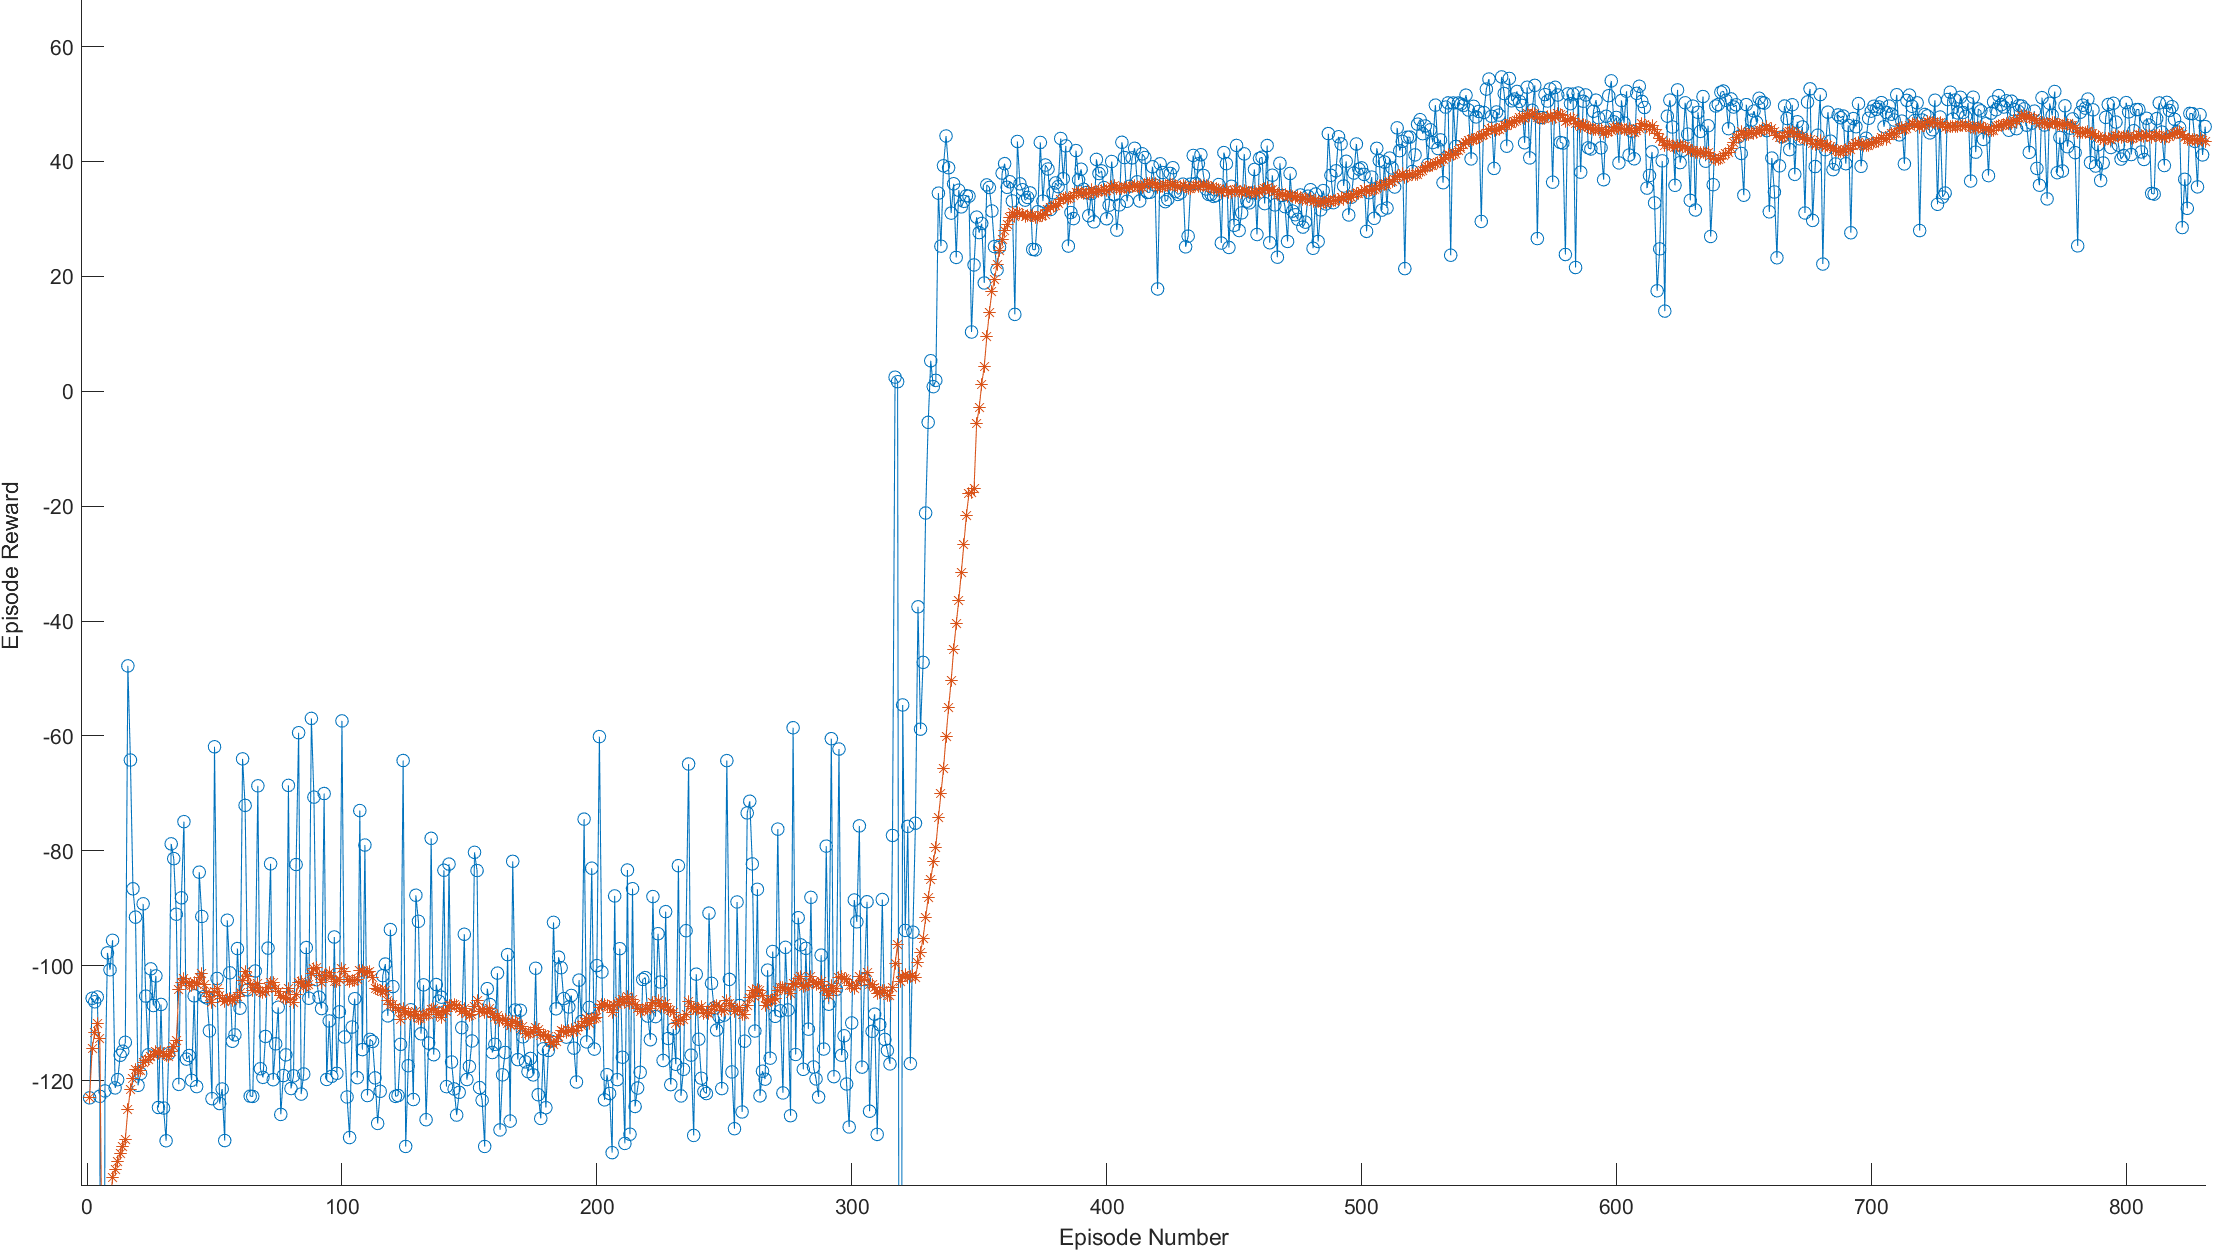
\includegraphics[width=12cm]{images/Training}
	\caption{Training process}
	\label{fig:training}
\end{figure}

\subsection{Evaluation of the reward function}

[implementation of the AR(1) process, numerical integration of the
  model output (acceleration?): numerical scheme, update time etc]

\subsection{The reinforcement learning process}

[things to look out for]

[typical figure of increasing reward over \#steps, then saturation]

[number of steps, computing time]

[figure of following trajectory instance at the beginning and after
  saturation of the 
  learning process]


\section{Validation}

The goal is not to minimize some error measure as in usual
calibration/validation but to check if the driving style is safe,
effecetive, and comfortable. Reference for this is the reward function

\subsection{string stability}

many trained RL vehicles behind the AR(1) realisation

\begin{figure}
	\centering
	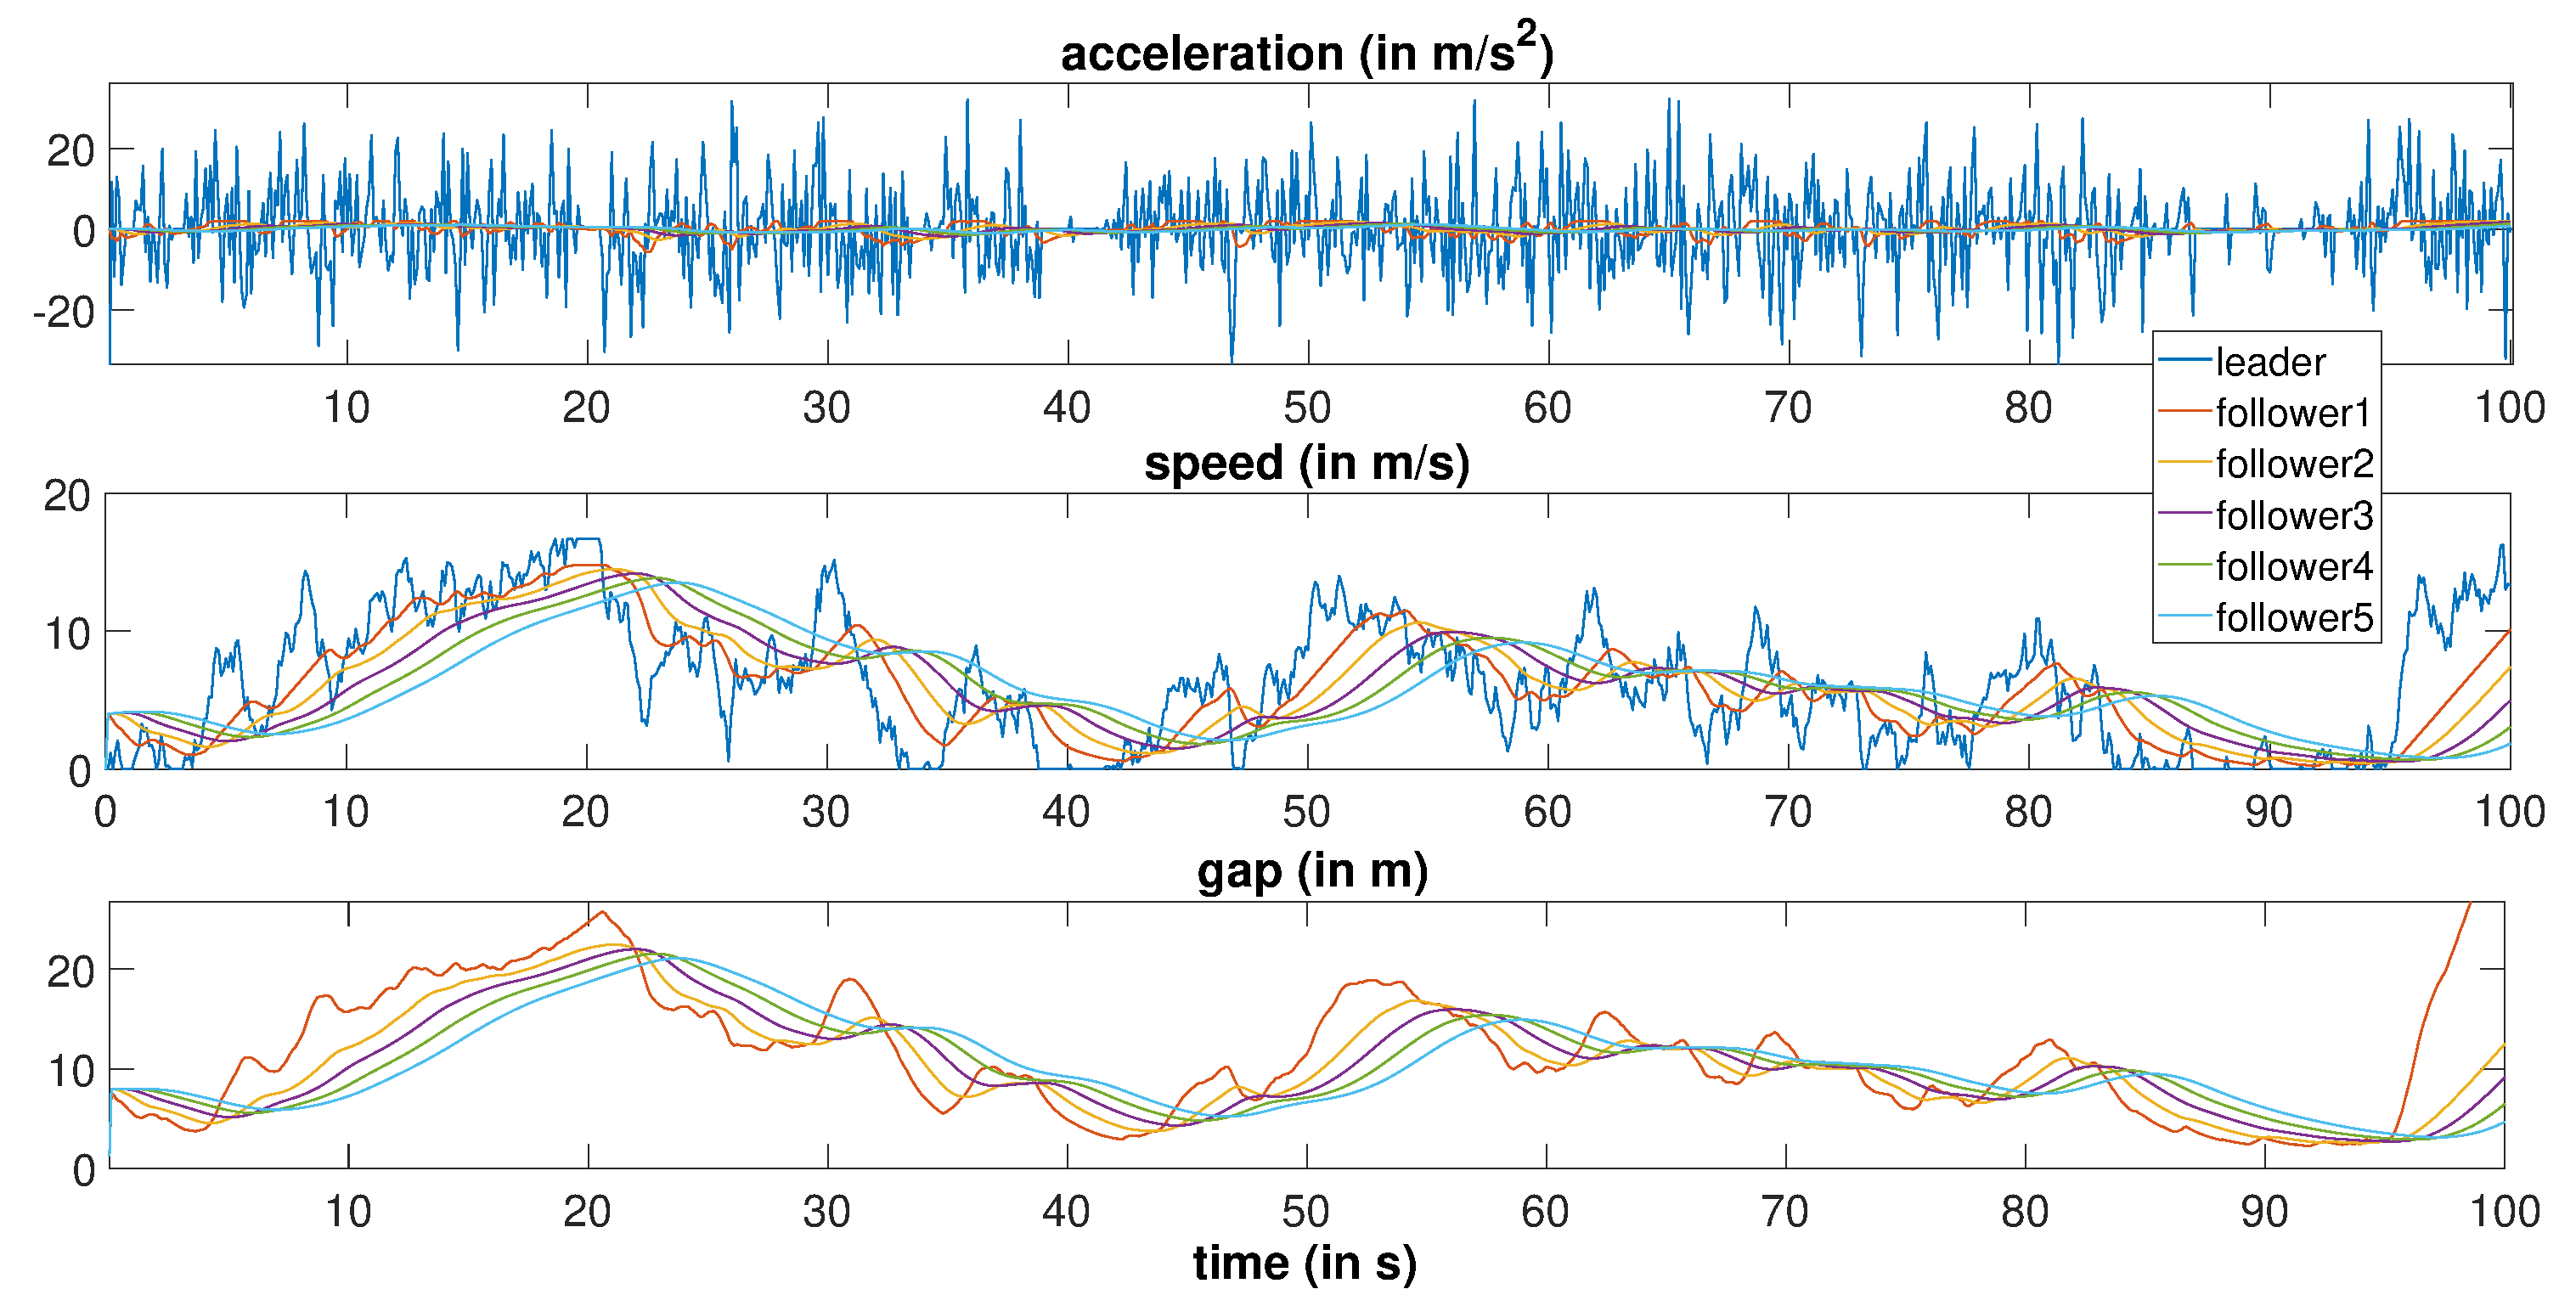
\includegraphics[width=12cm]{images/AR1Kolonne}
	\caption{}
	\label{fig:AR1Kolonne}
\end{figure}

\subsection{Response to an external leading vehicle speed profile}

[decribe profile with episodes of free driving, dynamic approaching,
  car-following, stopping, accelerating, and traffic waves]

\begin{figure}
	\centering
	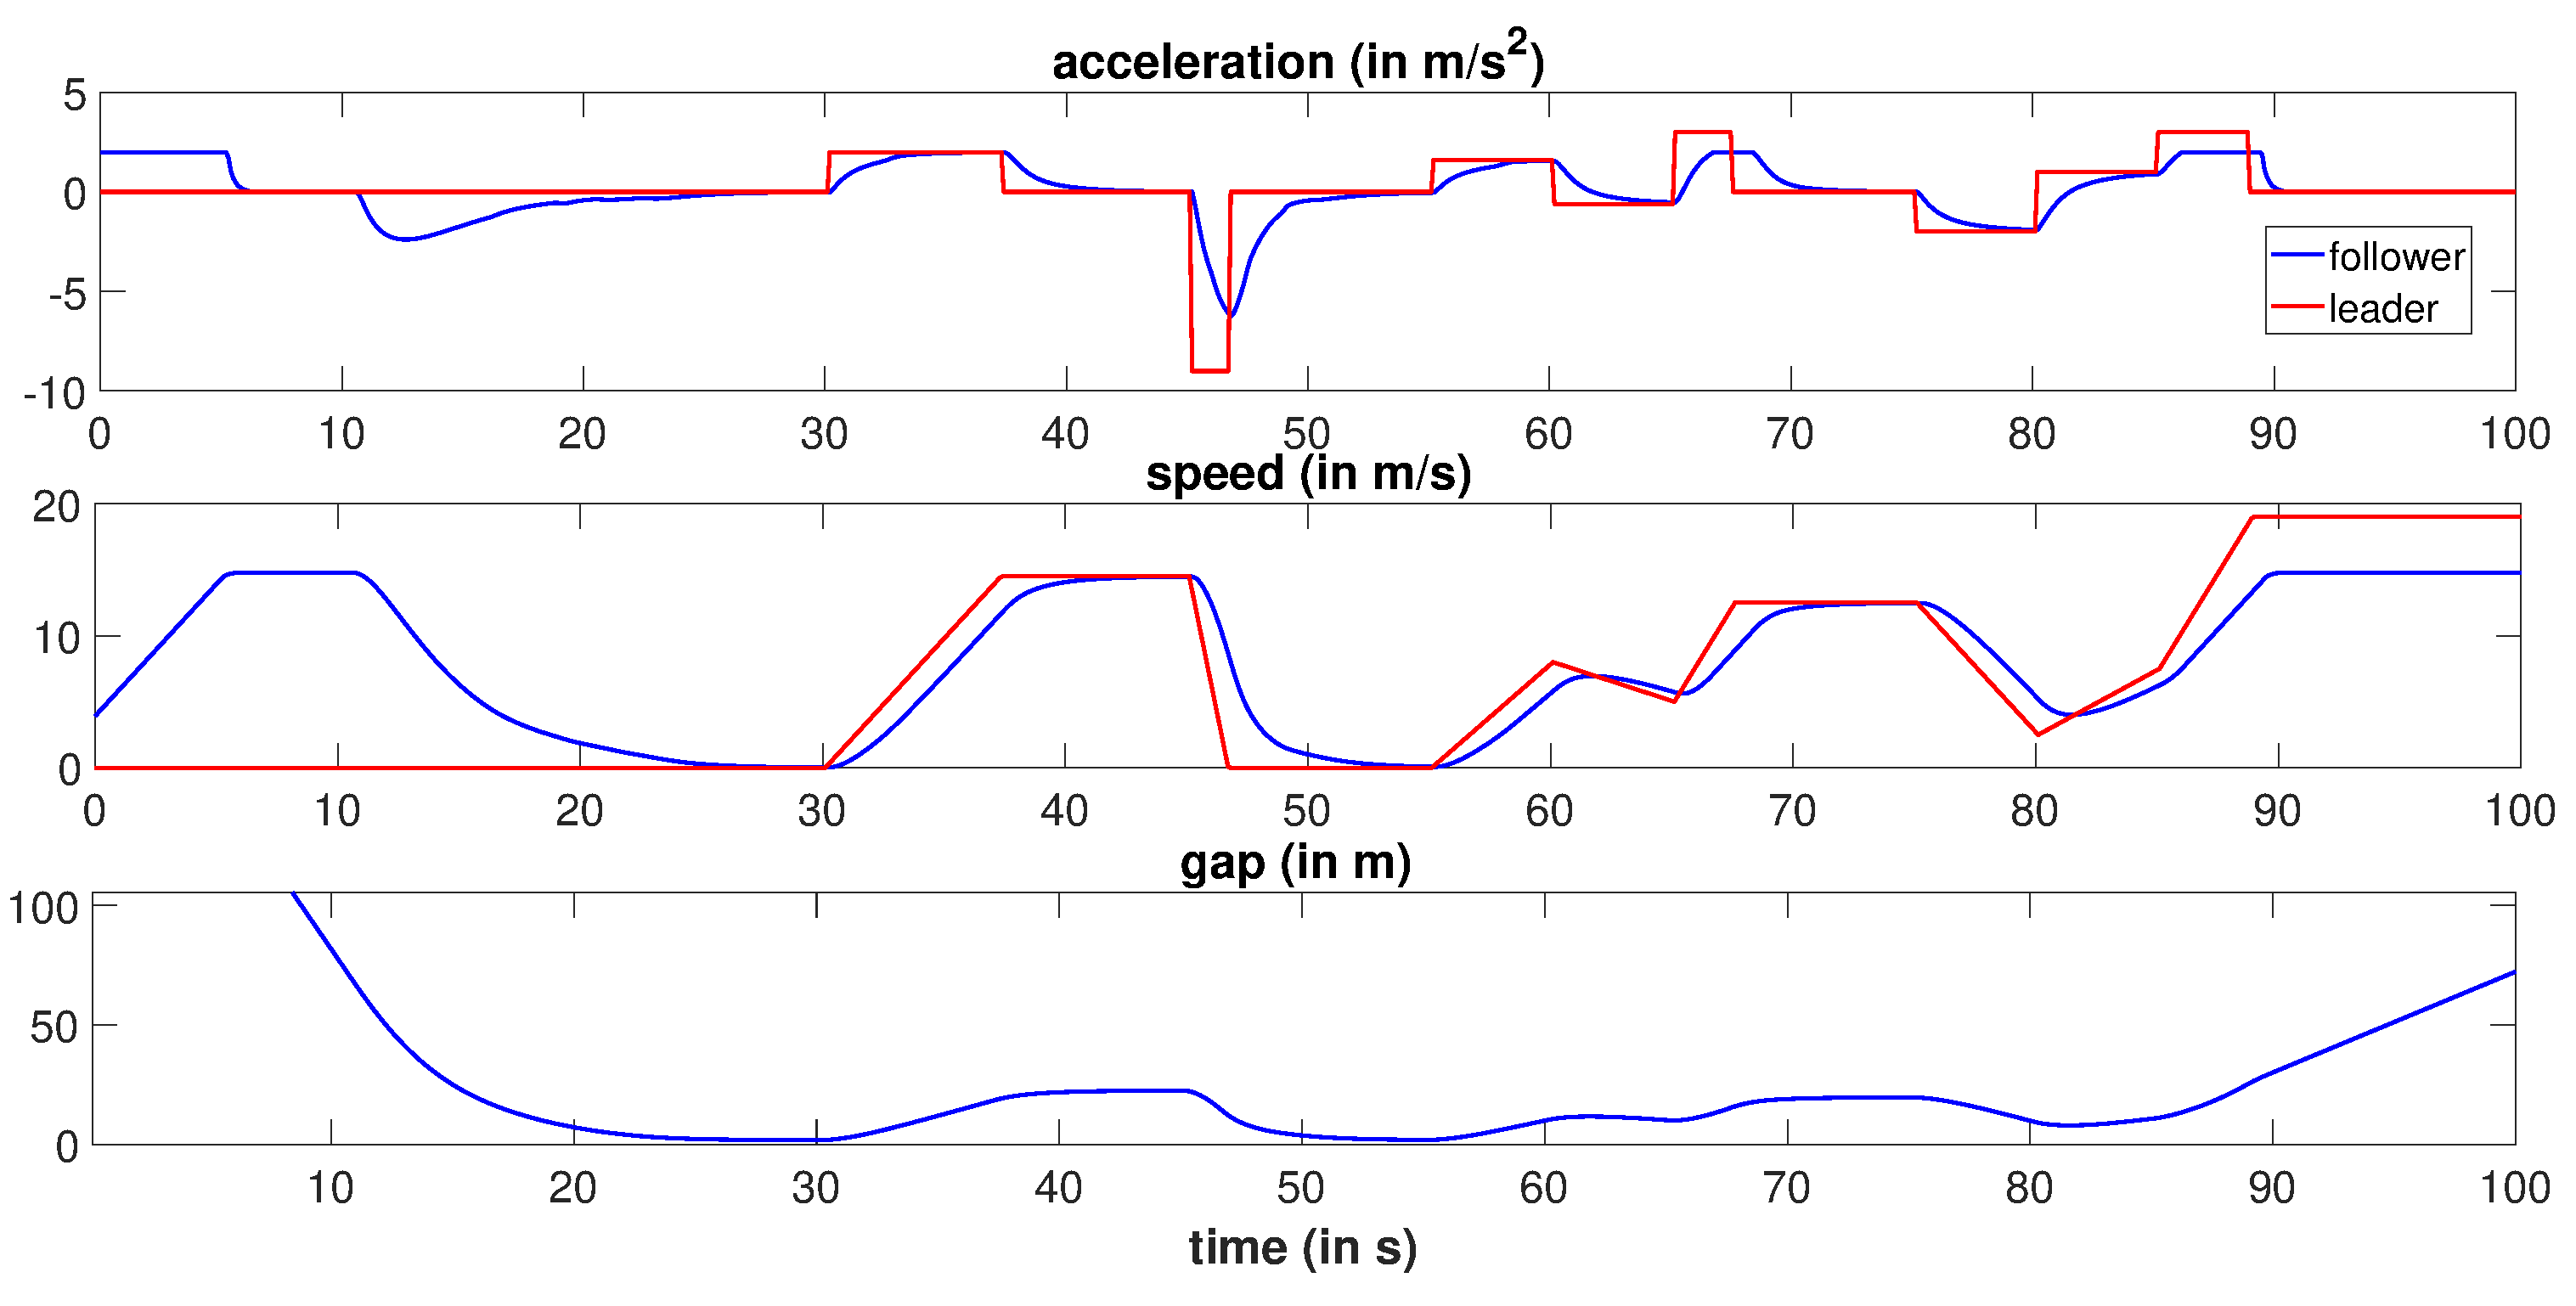
\includegraphics[width=12cm]{images/manipulatedLeader}
	\caption{}
	\label{fig:manipulatedLeader}
\end{figure}

[discussion: free: desired speed; following: desired time gap; dynamic
  situations: accelerations, desired and maximum  decelerations, jerk;
comfort: maximum accelerations, decelerations, jerk;
  safety: no crashs, minimum TTC; stability: string stable]


\subsection{Response to experimental leaders}

[describing the Napoli data]

[figure with several followers]

\begin{figure}
	\centering
	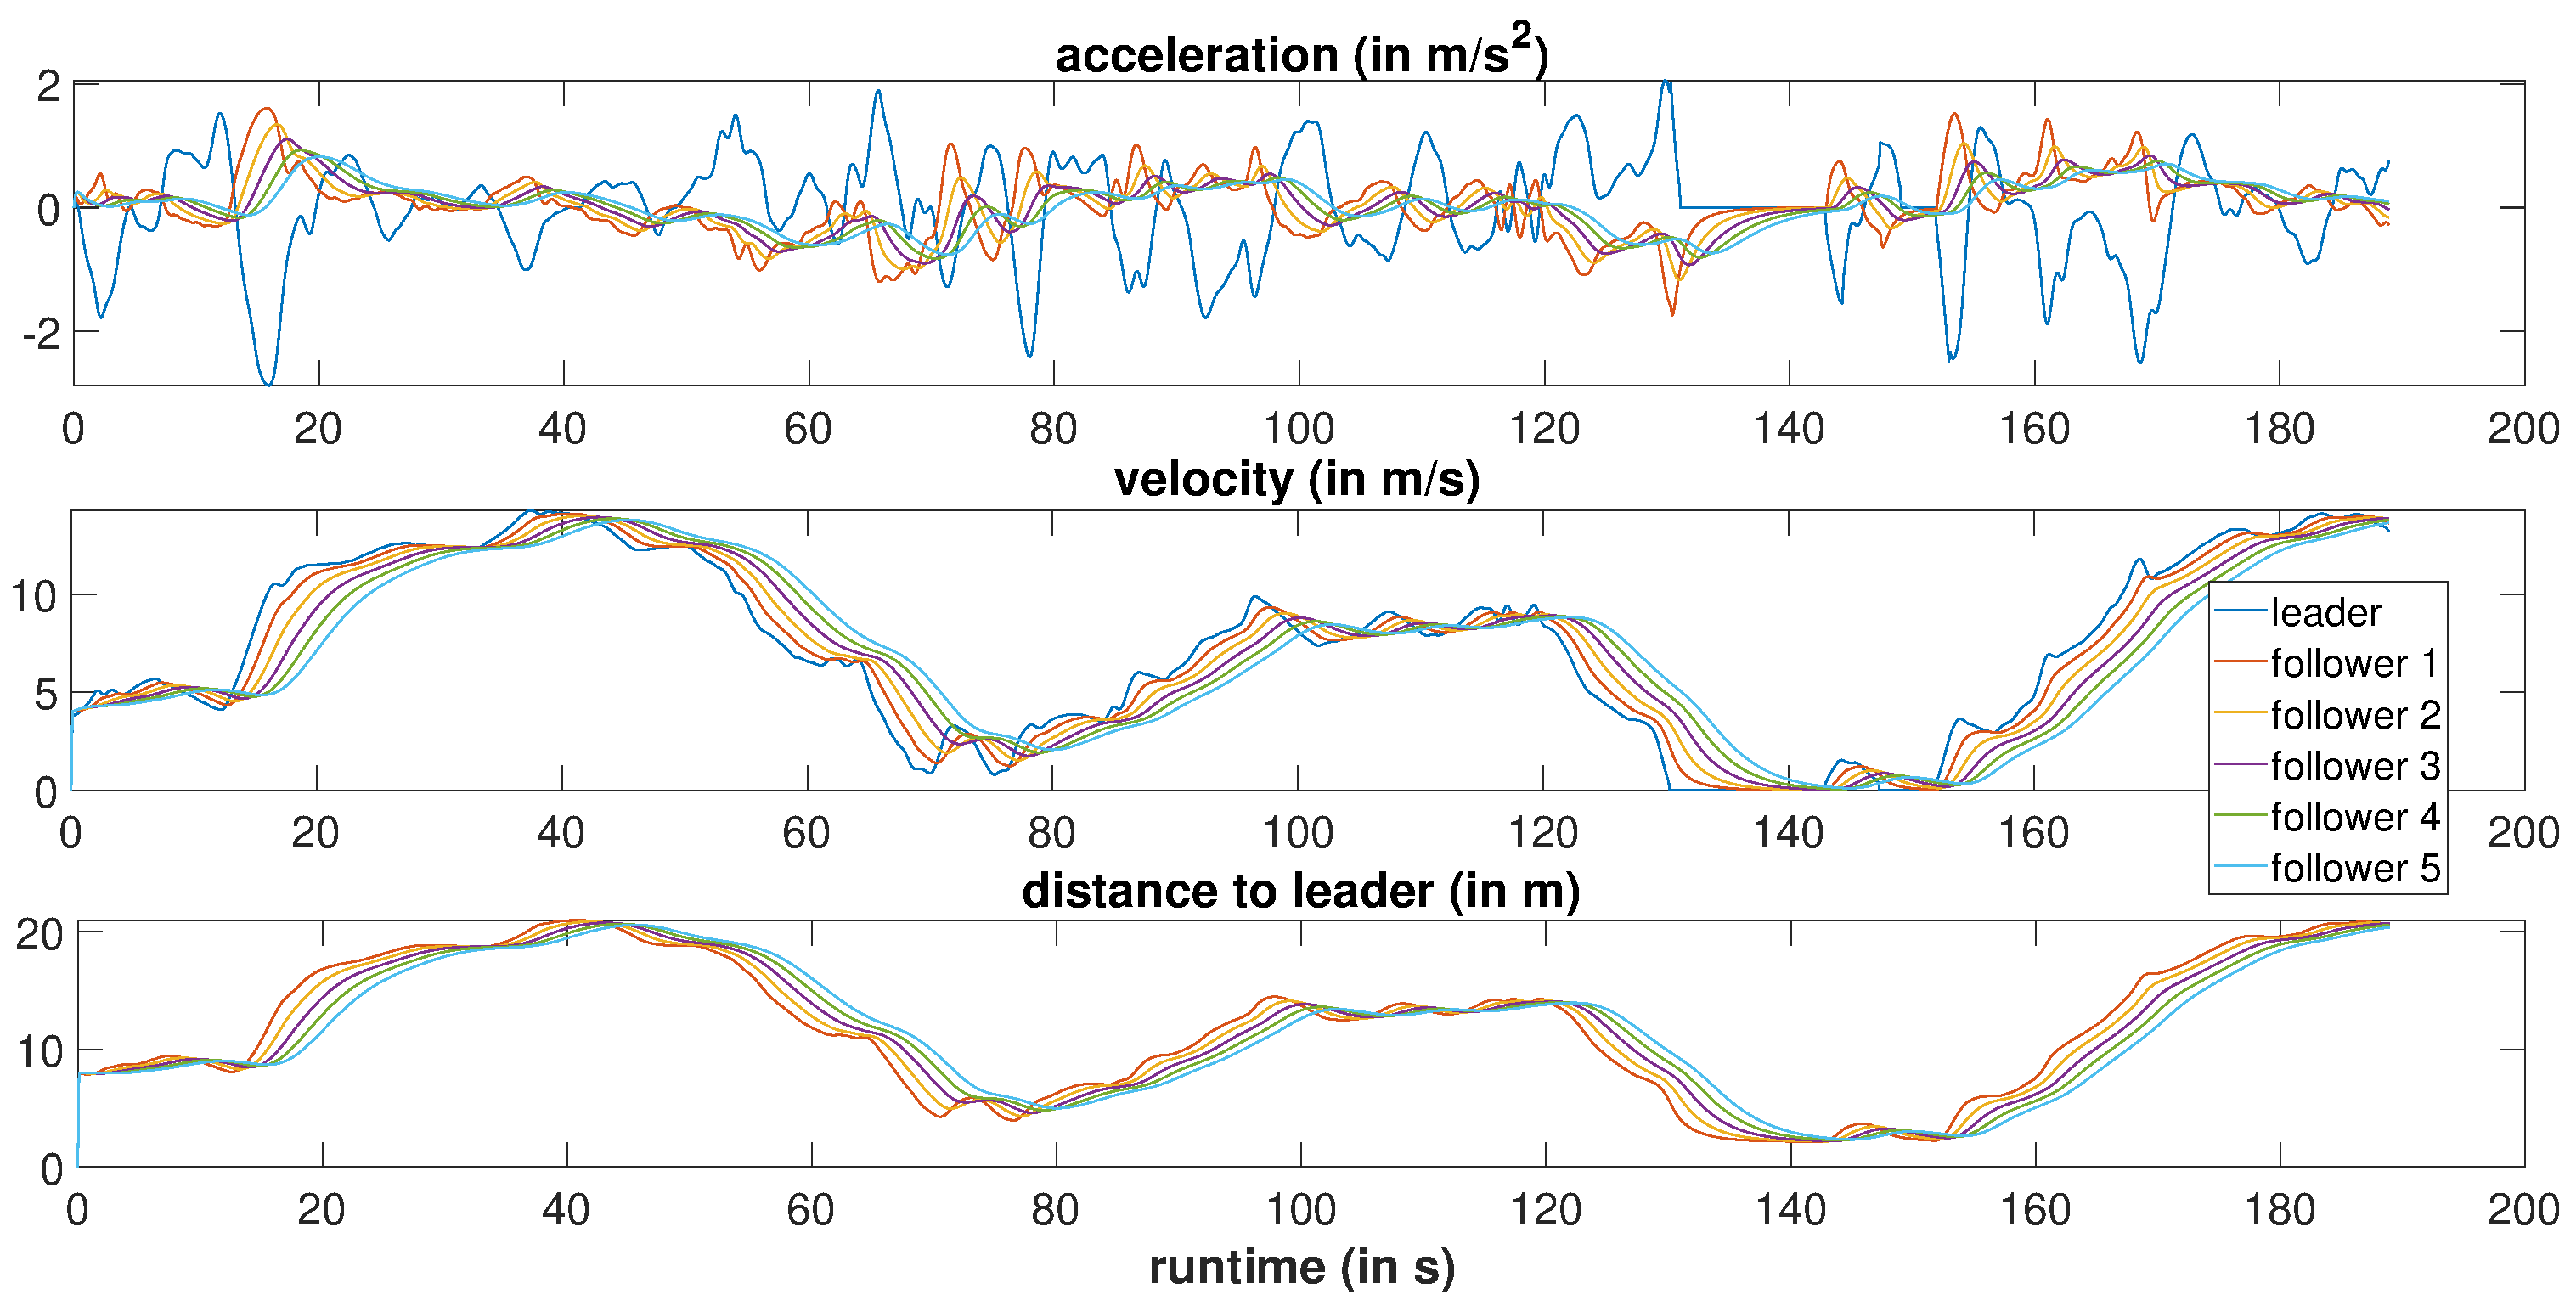
\includegraphics[width=12cm]{images/PunzoKolonne}
	\caption{}
	\label{fig:PunzoKolonne}
\end{figure}

[cross comparison with IDM calibrated to this set]
2x2 table; rows: RL model and IDM;
columns: reward function and calibration GoF (goodness-of-fit) function

\subsection{Repsonse of different driver characteristics to experimental leaders }

\begin{figure}
	\centering
	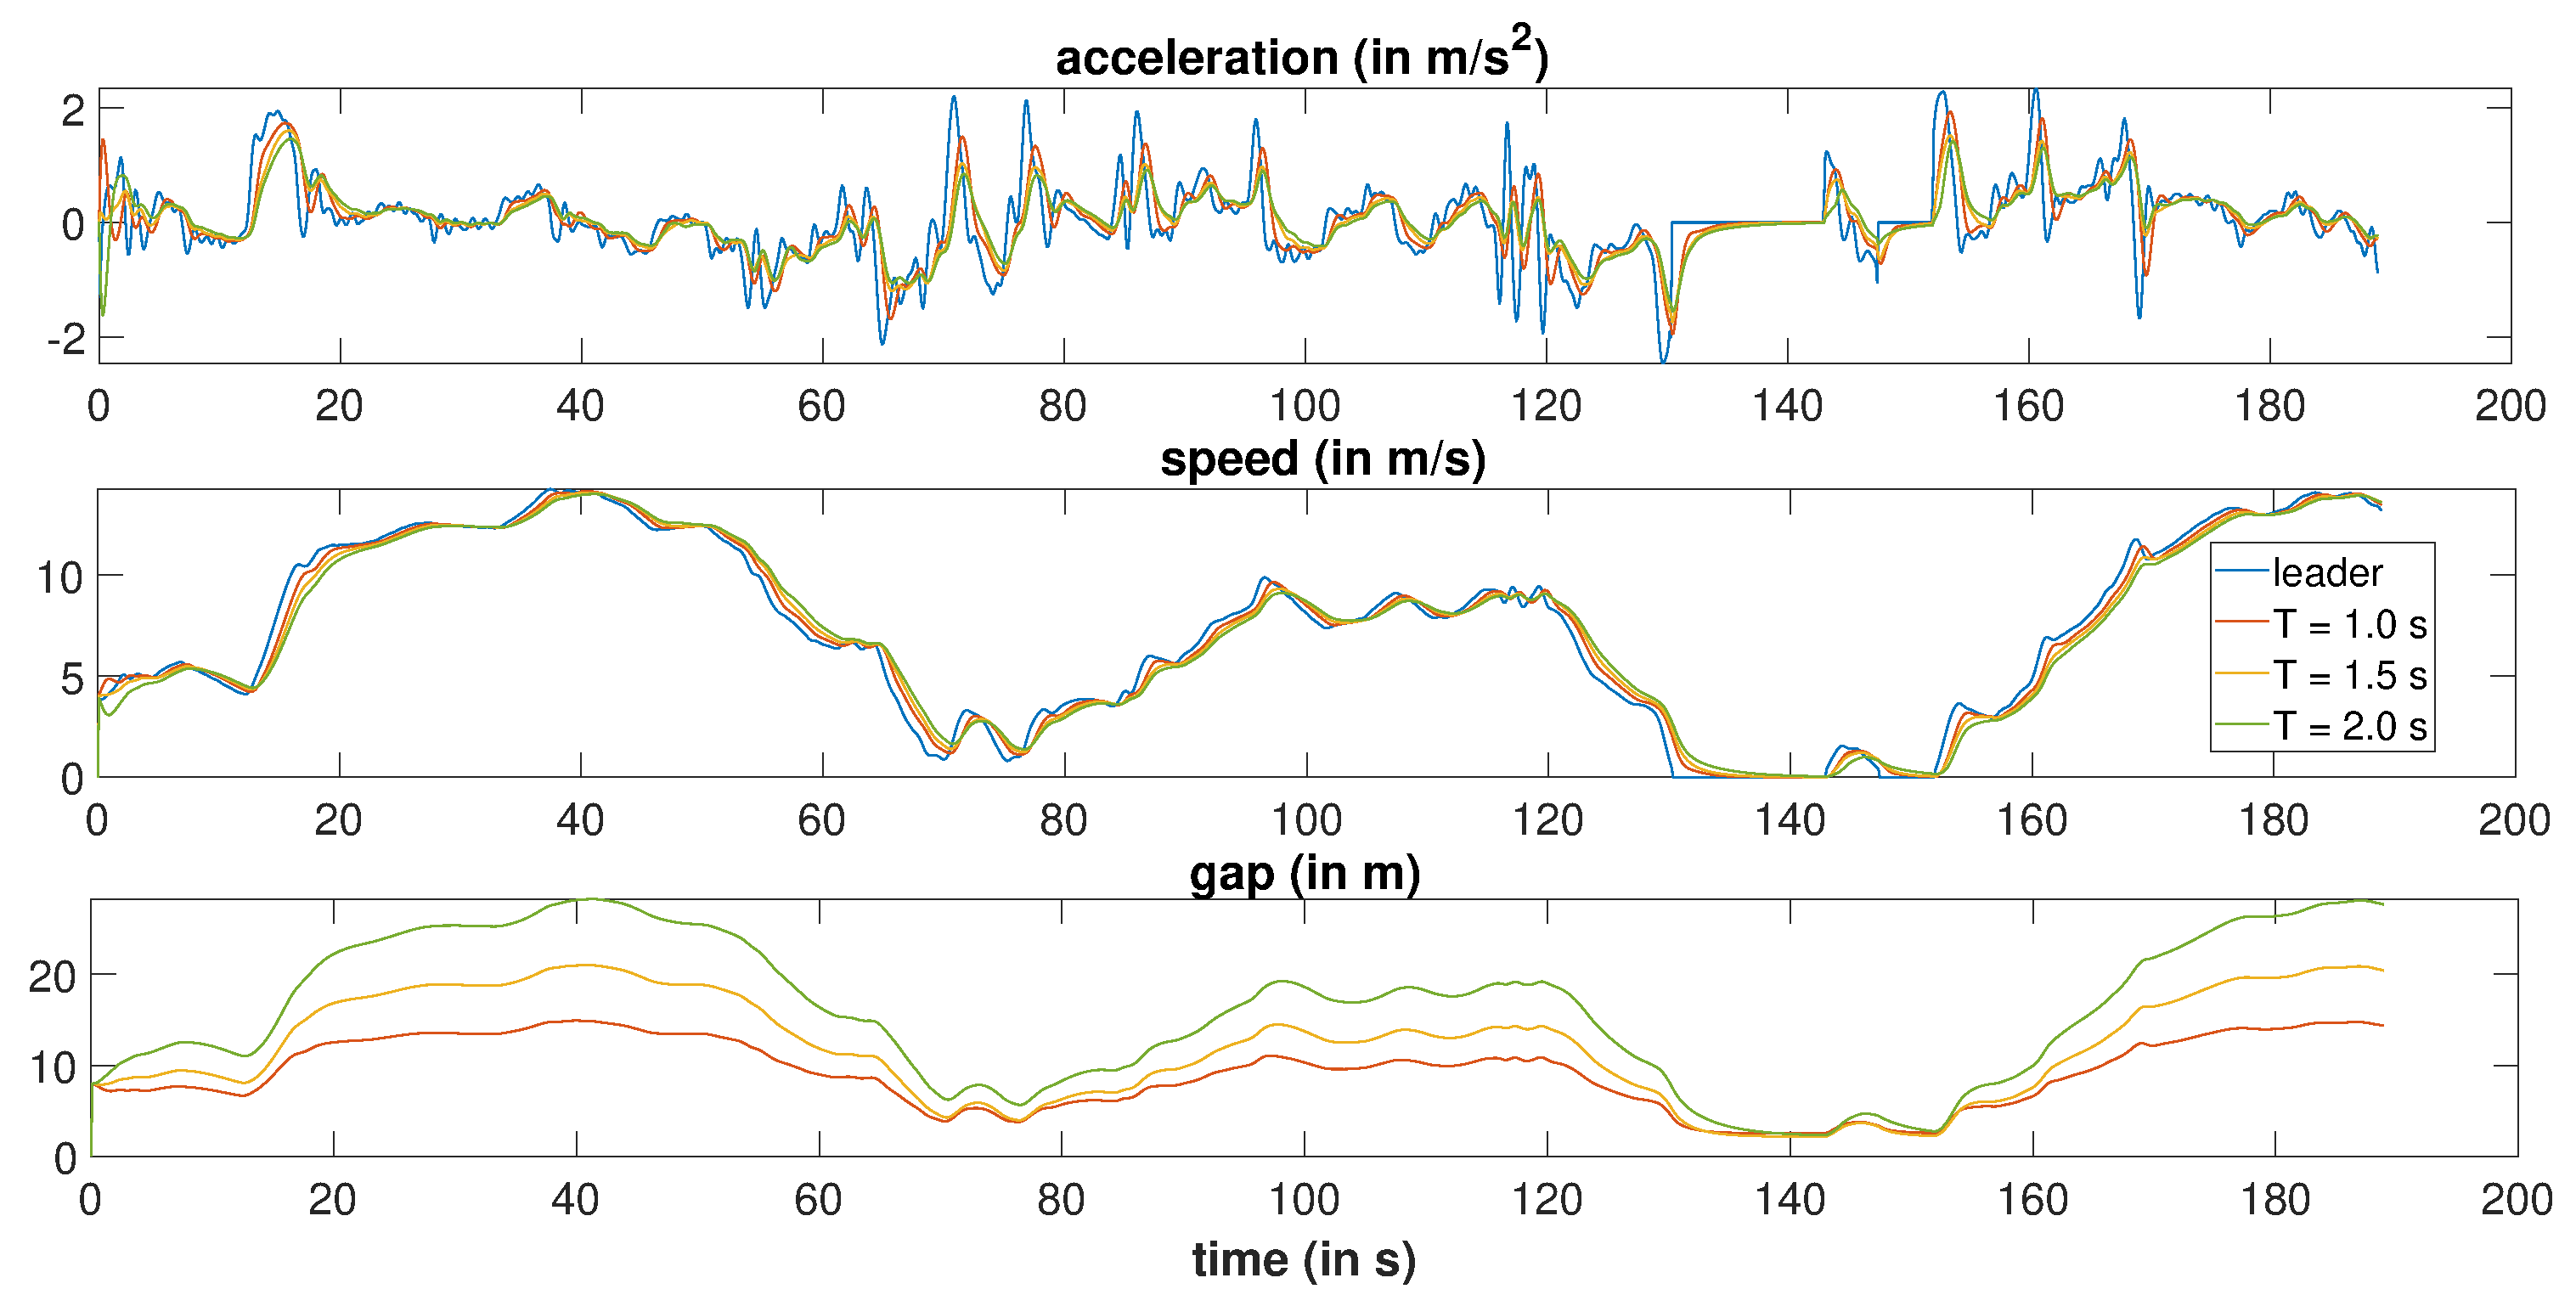
\includegraphics[width=12cm]{images/differentT}
	\caption{}
	\label{fig:differentT}
\end{figure}


\subsection{Simulation of collective phenomena}

[open system with speed-limit or on-ramp bottleneck (simplest vehicle
  dropping), increase inflow until breakdown to determine capacity,
  stability: no traffic waves, just congested traffic, maximum
  deceleration at the upstream jam front, propagation velocities]


\section{Conclusion/Discussion}

\section*{References}

\bibliography{RL_vehicles_references}

\end{document}
